%%%%%%%%%%
% [TODO] %
%%%%%%%%%%
% [ ] Mini-intro
% [ ] Anatomy of ASR system
% [ ] Parlato-hmm
% [ ] surfphono
% --- [ ] Add table with frequencies
% --- [ ] Results
% [ ] Mini-discussion

%%%%%%%%%%%%%%%%%%%%%%
% Chapter mini-intro %
%%%%%%%%%%%%%%%%%%%%%%

%%% Short BG
%\subsection{ASR tools as models of perception}


%%% Research question + alternatives


%%% Plan


%%%%%%%%%%%%%%%%%%%
% General methods % %
%%%%%%%%%%%%%%%%%%%

\section{Anatomy of our HMM-based speech recogniser}
In this chapter we used Hidden Markov Model (HMM)-based speech recognisers as models of human perception. 
Speech audio waveforms are transformed into a sequence of \textbf{acoustic vectors} $X_{1:T} = x_{1}, ..., x_{T}$ through the first step, called feature extraction. In the decoding phase that follows, the trained ASR system attempts to find the sequence of words $w_{1:L} = w_{1}, ..., w_{L}$ which is most likely to have produced the sequence of acoustic feature vectors $X$.
Mathematically, this equates to solving the following equation:

\begin{equation}
  \widehat{w} = \underset{w}{arg\,max} \left \{  P(w|X)\right \}
  \label{eq_hmm_dec_post}
\end{equation}

Put into Bayesian terms, this represents computing the posterior probability $P(w|X)$ of all combinations of words, given the acoustics, and retrieving the index of the most probable one: the decoder selects the sequence of words $w$ with highest posterior probability given the acoustic evidence $X$. However, due to the recursive and compositional nature of language, it may be difficult to evaluate all possible combinations of words, in order to find the most probable one. As such, following Bayes's theorem, equation \ref{eq_hmm_dec_post} can be rearranged as:

\begin{equation}
  \widehat{w} = \underset{w}{arg\,max} \left \{  P(X|w)P(w)\right \}
  \label{eq_hmm_dec_post}
\end{equation}

The likelihood $P(X|w)$, given by the \textbf{acoustic model}, is the probability of the acoustics given the sequence of words. The prior $P(w)$, given by the \textbf{language model}, corresponds to the probability of the word sequence, and can be derived from frequency counts. These probabilities can be extracted by training our ASR system using annotated speech corpora.

In the field of ASR, Neural Network (NN)-based speech recognisers are the state-of-the-art. In spite of better performance of NN-based ASR systems, we decided to use more well-understood HMM-based recognisers. Indeed, before the decoding step, these models offer a clear separation between the acoustic model (AM; i.e., mapping between phoneme categories and acoustics) and the language model (LM; i.e., frequencies of word/phoneme sequences). This allowed us to test ASR systems with different LMs while keeping the AM constant, as well as adapting LMs to mimic the experimental paradigms used when testing human participants. Importantly, unlike NNs which are often qualified as ``black boxes'', we are able to better understand and analyse how the ASR system processes acoustic input. 
We will now present the components of an HMM-based ASR system, as depicted in Figure \ref{fig:hmm_architecture}, in more detail.

\begin{figure}[htb]
\centering
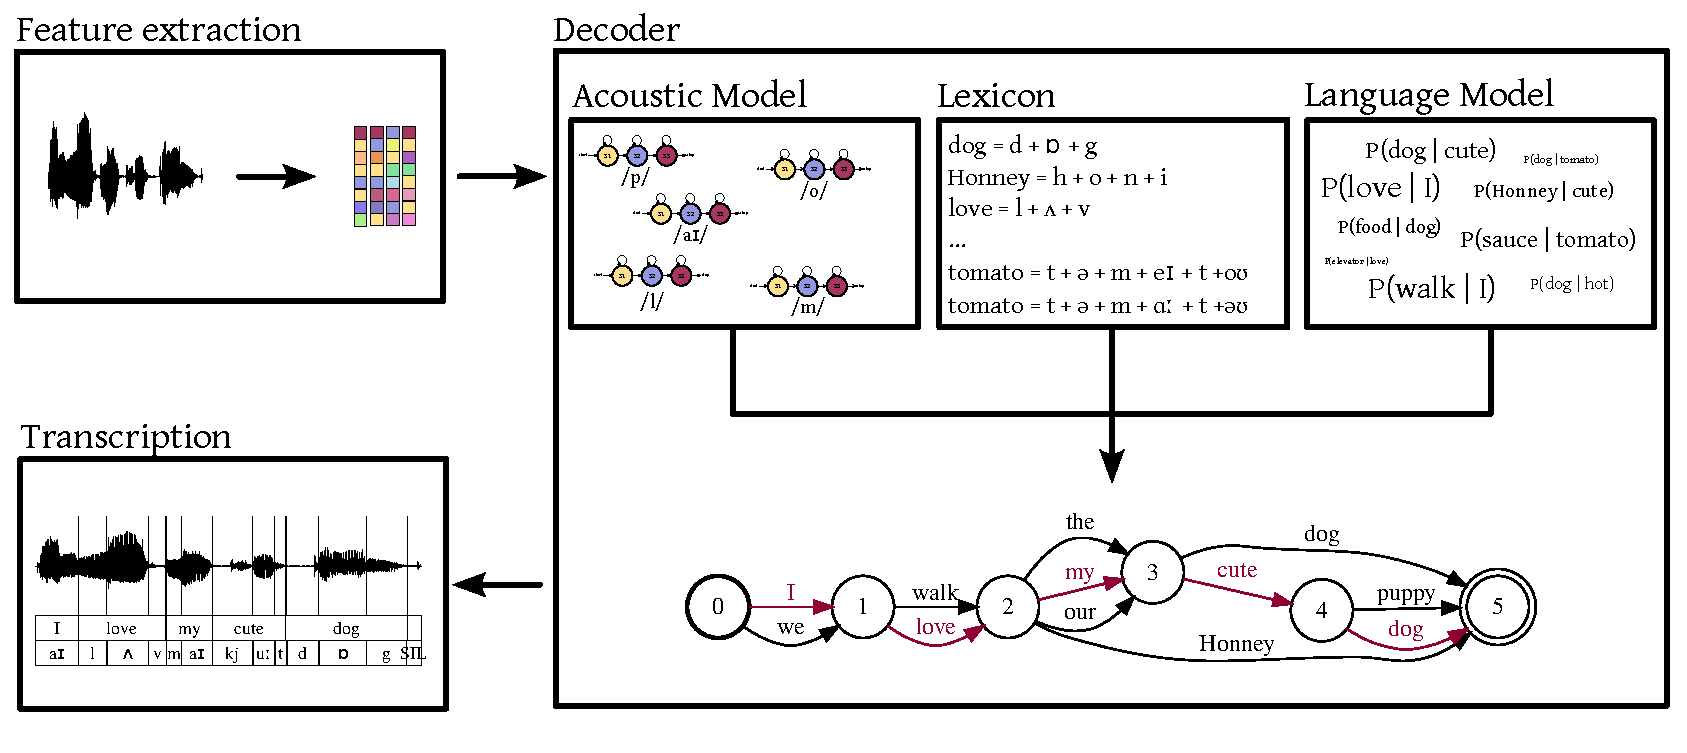
\includegraphics[width=1\linewidth]{chapter03/hmm_all.pdf}
\caption{\textit{Architecture of our ASR system, including its input (acoustic features) and output (transcription).}}
\label{fig:hmm_architecture}
\end{figure}

\subsection{Corpora}

In order to train and test our ASR system, we required transcribed speech corpora. These corpora consisted of speech recordings which have been annotated; for each utterance, we have a more or less detailed transcription of what was said.
While the ideal annotation is one for which phoneticians have provided phoneme categories (or even phones), as well as their boundaries, often we might only have access to by-utterance annotations where we are only provided with a sequence of words/phonemes for each utterance. In these cases, we rely on forced alignment to automatically find phoneme boundaries.

In the following sections we have trained ASR systems with different ``native'' languages, namely Japanese (JP) and Korean (KR). These languages were of particular interest because of their relatively restrictive phonotactic constraints with regards to consonant clusters, as well as the availability of corpora of spontaneous speech, which we will now present. 

\paragraph{Corpus of Spontaneous Japanese (CSJ)}
As the name suggests, the CSJ \cite{maekawa2003} contains recordings of spontaneous Standard Japanese. The corpus is composed of two subparts: (1) academic presentation speech (APS), which consists of live recordings of academic presentations, and (2) simulated public speech (SPS), where speakers presented everyday topics in front of a small audience. For our models we only kept SPS, which is more representative of everyday conversations at the level of the lexicon, and has a more balanced population than the young male-dominated APS.
Recordings were manually transcribed by native speakers of Japanese. Phoneme boundaries were {\color{red}manually adjusted, however this alignment was not used when our models, as it was overwritten by forced alignment}.
Our subset of the corpus contained $400,547$ utterances produced by $594$ speakers\footnote{We used utterances from the same speakers for the validation and test sets, but their data was not used during model training. The same was done for the Korean model.} ($331$ female, $263$ male), with an average of $674.3$ utterances per speaker. The division of the corpus across training, validation, and test set are shown in Table \ref{tab:hmm_csj}.

\begin{table}[htb]
\centering
\caption{Datasets used for training and evaluating the Japanese ASR system.}
\label{tab:hmm_csj}
\vspace{0.25cm}
\begin{tabular}{rrrrrr}
  \toprule
      & Proportion &\# Utterances & Duration & \# Speakers &  \\ \midrule
  train & $80\%$ &  $322,208$            & 6 days, 8:26:33     &   475          &  \\
  valid & $5\%$ &  $19,566$         &  9:12:03    &   119          &  \\
  test  & $15\%$ &  $58,773$        &  1 day, 3:19:14    &  119           & \\ \bottomrule
\end{tabular}
\end{table}

\paragraph{Korean Corpus of Spontaneous Speech (KCSS)}

The KCSS \cite{yun2015} consists of recordings of spontaneous Seoul Korean. Forty speakers aged $10$ to $49$ ($5$ female speakers and $5$ male speakers per decade) were recorded in a quiet room, for approximately 1 hour each. Speech was ellicited through questions related to the speakers' personal opinions, habits, acquaintances, etc.      
Recordings were manually transcribed by native speakers of Korean. We used phonetic transcriptions faithful to actual pronunciations which, for instance, include phonetic reduction (akin to \textit{yesterday} being transcribed as \textipa{/jESeI/} instead of the canonical \textipa{/jEst\textrhookschwa deI/}). Transcriptions include {\color{red}manually adjusted} phoneme boundaries, as well as word syllabification. {\color{red}[NOTE]: \%WER for mono-pitchT-1000 is 81.1\% with forced alignment and ... 99.3\% when ``using the manual alignment''!!!! For this latter, many words as transcribed as ``$<$unk$>$'', so something is very wrong. Maybe at the level of the ali.*.gz files?}
The corpus contains $57,504$ utterances produced by $40$ speakers (as explained above), with an average of $1,437.6$ utterances per speaker. The division of the corpus across training, validation, and test sets is shown in Table \ref{tab:hmm_kcss}.

\begin{table}[htb]
\centering
\caption{Datasets used for training and evaluating the Korean ASR system.}
\label{tab:hmm_kcss}
\vspace{0.25cm}
\begin{tabular}{rrrrrr}
  \toprule
      & Proportion & \# Utterances & Duration & \# Speakers &  \\ \midrule
  train & $80\%$ &  $46,208$ &   18:58:15   &   $32$    &  \\
  valid & $5\%$ &  $2,824$ &  1:16:39  &  $8$  &  \\
  test  & $15\%$ &  $8,472$ & 3:54:15   & $8$    & \\ \bottomrule
\end{tabular}
\end{table}

\subsection{Features}
In order for our ASR systems to be able to use speech as input, it is necessary to perform signal analysis. This procedure transforms the continuous raw speech waveform into sequential speech features. This latter form ensures a more compact representation of the information in speech, with modifications that enhance phonemic contrasts and better approximate how speech is processed by the human cochlea. In this work we used Mel-frequency cepstrum coefficients (MFCC), traditionally used for HMM-based ASR systems.

\begin{figure}[htb]
\centering
%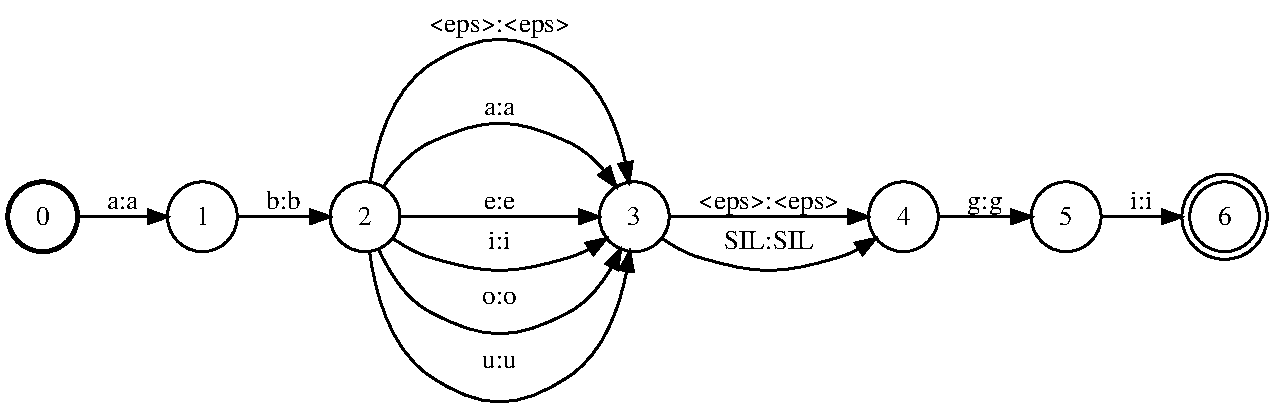
\includegraphics[width=0.8\linewidth]{chapter03/parlato_hmm_Gfst.pdf}
\caption{{\color{red}\textit{[Is this necessary or is the text enough?] Processing stages required to obtain MFCCs.}}}
\label{fig:hmm_features}
\end{figure}

Speech is recorded with a microphone; the continuous audio signal is digitalized at a sampling rate of 16kHz.
The audio is then segmented into frames of 25 ms, with a shift of 10 ms between the beginning of each frame. By using frames, we make the assumption that the signal is stationary, and we apply the following proccessing steps to each frame, using Kaldi \cite{povey2011}:

\begin{enumerate}
\item Pre-processing: The data is extracted and pre-processed (dithering, pre-emphasis, and DC offset removal).
\item Windowing: The data in the 25 ms frame is multiplied by a tapered window (Hamming window), to avoid discontinuities at the edges of the segment.
\item Spectral analysis: By applying a Fast Fourier Transform (FFT), we find out how much energy there is at each frequency band for this frame.
\item Nonlinear frequency scaling: In order to compensate for the fact that human hearing is less sensitive to higher frequencies, frequencies are mapped onto a Mel scale, which is linear until approximately 1000 Hz and logarithmic afterwards. This is done by applying a mel-filter bank with 23 bins, which are equally spaced in the mel-frequency domain. Each filter summarises the amount of energy in a section of the range of frequencies. 
\item Cepstral analysis: The log of the energy in each bin is computed, from which we take the cosine transform. We keep 13 MFCCs, including $c_{0}$, the zeroth coefficient which represents the average of the log-frequency of the bins \cite{gales2008}.
  \item Cepstral liftering: Coefficients are scaled, ensuring that they have a reasonable range.
\end{enumerate}

We therefore obtain 13 MFCCs that summarise the information at each frame of audio. To these coefficients, we add 3 coefficients carrying information about pitch: normalized-pitch, delta-pitch, voicing-feature\footnote{Information about pitch was added because of its contrastive relevance in Japanese at the lexical level (i.e., pitch accent) and in Korean at the phonemic level (e.g., tonogenesis in the three-way contrasts of plosives). In practice, adding pitch features resulted in a slight improvement of model performance in Japanese (from $41.3\%$ WER to $39.6\%$; acoustic model with 6000 Gaussians).}.
To these 16 static features we add their respective dynamic features ($\Delta$ and $\Delta^2$) that describe the evolution of the coefficient values over time. 
Coefficient values are then standardised using Cepstral Mean Variance Normalisation (CMVN); for each speaker the distribution of each coefficient's values has a mean value of zero and a variance of one. 

\subsection{Acoustic model}

Now that we have extracted the acoustic features for the labelled utterances in our corpus, we are able to train the acoustic model (AM). Recall that the AM gives the likelihood $P(X|w)$, which corresponds to the probability of the acoustics given the sequence of words $w$.
In order to simplify things, let's not view an utterance as a sequence of words which are sequences of phonemes themselves, but directly as a sequence of phonemes. Then, we consider the probability of the acoustics $X$ given the sequence of phonemes $W$.
Phonemes are not static objects but trajectories of the acoustic signal, of varying duration. By using Hidden Markov Models (HMM), we can approximate these trajectories as sequences of static states. A priori, the more states, the better the approximation. However, empirically it has been assessed that having three states is a good compromise for ASR systems. Following this, we chose to model phonemes as 3-state HMMs, where the states correspond, respectively, to the beginning, middle, and end portions of the phoneme. This is particularly relevant for phonemes that can be viewed as sequences of discrete articulatory events with distinct acoustic signatures, such as plosives (e.g., \textipa{/p/}) which are often described as an airway closure, followed by a period of occlusion and an optional release. Additionally, the separation into three states allows to account for the fact that the acoustics of the beginning and end of a phoneme may be differently affected by neighbouring phonemes (i.e., coarticulation) in comparison to the medial part.

As their name suggests, HMMs follow a Markovian process; the value of a state only depends on the value of the previous state. The transitions between states are defined by transition probabilities not only between adjacent states, but also within a state itself (i.e., self-loops). These transition probabilities are defined during AM training, based on the transitions between frames in the training corpus. While the duration of phonemes cannot be explicitly learned by the acoustic model, they are implicitly reflected by the transition probabilities in the self-loops: for a given state, the higher the self-loop probability, the longer the model will ``remain'' at said state and the longer the sequence of acoustic vectors assigned to the corresponding phoneme. A simplified illustration of a phoneme HMM is shown in Figure \ref{fig:hmm_3state}.

\begin{figure}[htb]
\centering
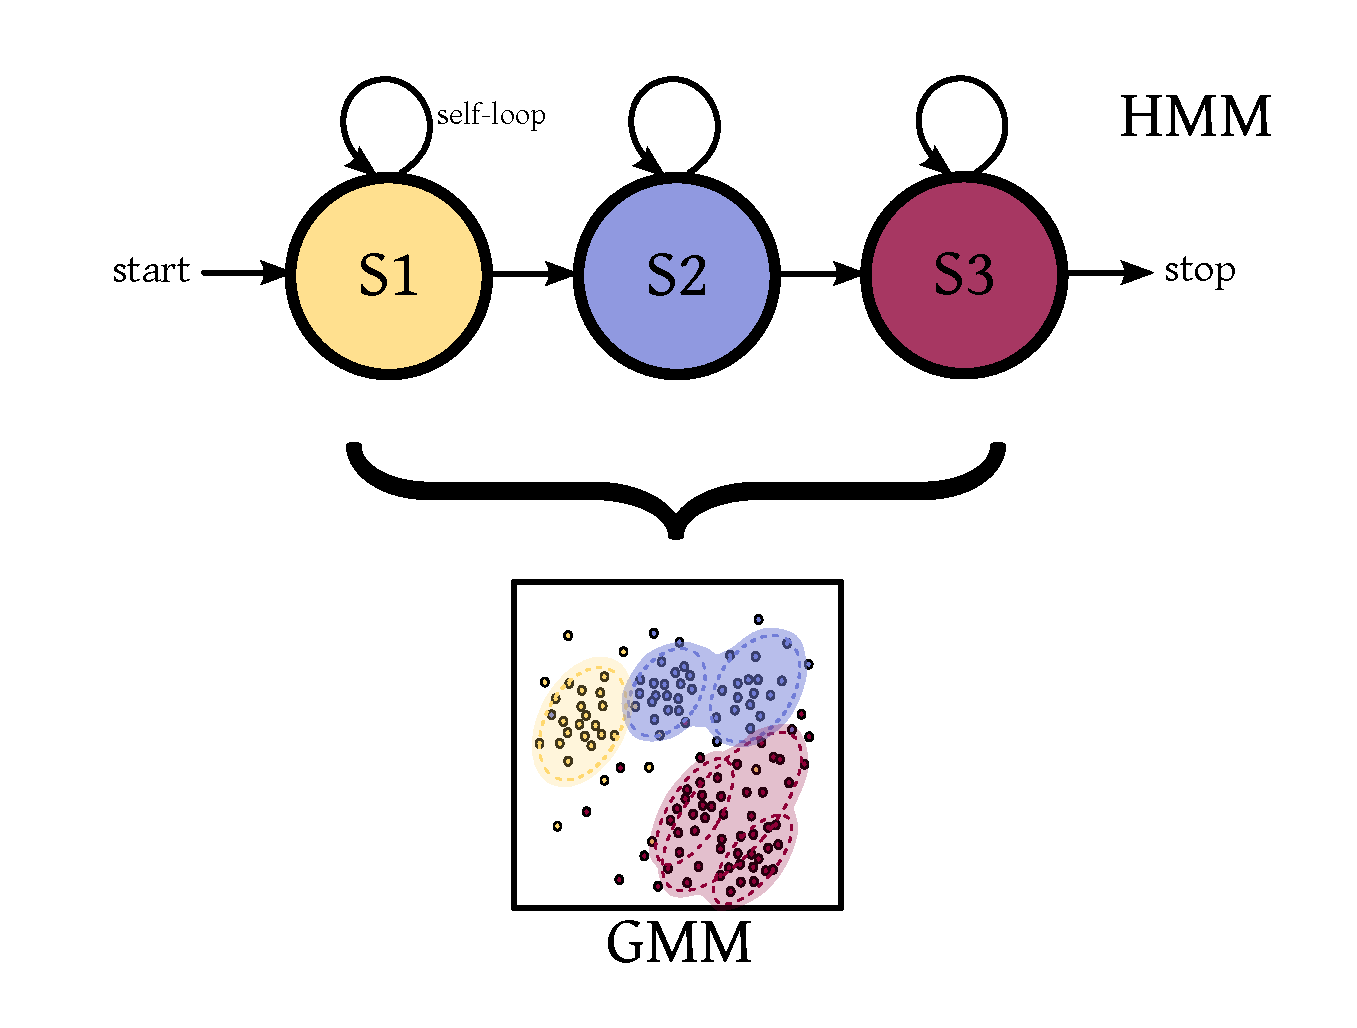
\includegraphics[width=0.6\linewidth]{chapter03/hmm_3state.pdf}
\caption{\textit{Left-to-right 3-state phoneme HMM with simplified 2-dimensional GMMs (one per state). Start and stop states connect the phoneme with the previous and next phoneme, respectively.}}
\label{fig:hmm_3state}
\end{figure}

In sum, each phoneme is modelled by a left-to-right 3-state HMM. But what exactly is a state? Our acoustic models are HMM-GMMs, where GMM stands for Gaussian Mixture Models. For each phoneme our 48-dimensional feature vectors define a 48-dimensional space where GMM for the three states are embedded. During training, the acoustic model will have placed individual acoustic frames on this space, based on the values of their feature vector. In other words, acoustic frames from each phoneme portion will occupy a certain part of this space. For each state, we can parametrically define the space covered using mixtures of Gaussian distributions (the aforementioned GMMs). Indeed, GMMs are universal approximators of densities when given enough components. To do this, the model will have fitted a number of diagonal Gaussian distributions to approximate the distribution of datapoints corresponding to each phoneme state. The number of Gaussians allocated to each phoneme state depends on the total number of Gaussians made available to the model, and the complexity of the distribution of the frames in the space. Once that the GMMs are defined, the AM is able to tell us, for any new frame, the likelihood that the frame originated from each GMM (i.e., phoneme state).  \\     


{\color{red} $<$OLD VERSION$>$
\subsubsection{Estimating Gaussian distributions}
We have 48-dimensional vectors (i.e., our acoustic features), as well as their accompanying transcriptions, as input for our acoustic model. As such, for each acoustic frame, we know the identity of the phoneme that it constitutes. Therefore, we have access to a variety of feature vectors which we can group by phonemic category. Using these distributions of acoustic vectors, we are able to represent each phoneme as a multivariate Gaussian distribution with 48 dimensions. During training, our acoustic model learns what each multivariate Gaussian distribution looks like for each phoneme by estimating the means and covariance matrices necessary for defining said distributions.
Then, the AM is able to tell us, for any new frame $x$, $P(x|w_{l})$ the likelihood that the frame originates from each multivariate distribution (i.e., phoneme) $w_{l}$. However, this assumes that a (multivariate) Gaussian distribution will be sufficient to model the distribution of our data. This is a strong assumption but it is made unnecessary by replacing multivariate Gaussian distributions with Gaussian Mixture Models (GMM).

\subsubsection{Adding Gaussian Mixture Models (GMM) into the mix}
Indeed, given enough components, GMMs are universal approximators of densities. We can therefore represent each phoneme not as a single multivariate Gaussian but as a mixture of multiple ones, relaxing the normality assumption. Similar to the single multivariate case, training consists of teaching the acoustic model what the distribution of exemplars of each phoneme looks like. The AM can then fit mixtures of Gaussians to fit these (non-Gaussian) distributions. When presented with a new frame, the AM can retrieve the likelihood that it originates from each GMM (i.e., phoneme). However, this type of acoustic model does not take into consideration the sequential nature of speech. Here is where Hidden Markov Models (HMM) come into place.   

\subsubsection{Modelling sequences with HMMs}
Before even mentioning how different phonemes are connected to each other in HMMs, our first modification will be within the representation of an individual phoneme itself. While in the previous paragraph each phoneme was a GMM, now we represent a phoneme by a sequence of three GMMs, called \textbf{states}. In a left-to-right model such as ours, the three states are disposed sequentially (i.e., it is only possible to go from state 1 to state 2, and from state 2 to state 3) and they correspond to a description of phonemes unfolded in the time domain. Shifting to a three-state representation allows us to better handle the variability in phoneme production due to coarticulation; indeed, while state 2 represents the more stable, medial portion of a phoneme, states 1 and 3 will be subjected to more diversity due to surrounding phonemes. Additionally, some phonemes are better represented by a sequence of steps rather than a stationary description of their acoustics. For instance, plosives such as \textipa{/p/} are often described as sequences of an airway closure, followed by a period of occlusion and an optional release.

In previous paragraphs we mentioned that, during training, our AM was learning the GMMs for all phonemes based on the corpus data. Now that we represent phonemes as three-state HMMs, our AM also needs to learn the transition probabilities, within states (i.e., self-loops) and between adjacent states. How do we go from isolated phonemes to sequences of phonemes? Phoneme HMMs are simply chained together, meaning that the AM also learns the transition probabilities between the last state and first state of a pair of phonemes.

Please note that HMMs follow a Markovian process; the probability of a state only depends on the state beforehand. Consequently, the duration of phonemes cannot be explicitly learned by the acoustic model. However, durations are implicitly reflected by the transition probabilities in the self-loops: for a given state, the higher the self-loop probability, the longer the model will ``remain'' at said state and the longer the sequence of acoustic vectors assigned to the corresponding phoneme.  \\
$<$/OLD VERSION$>$}

\subsubsection{Why not triphones?}
If the reader is already familiar with ASR systems, they may expect us to go a step further and no longer treat phonemes as units (i.e., monophones) but, instead, handle triphones. For this latter representation, an independent three-state HMM would be built for each combination of three phonemes. For instance, there would no longer be an HMM for \textipa{/p/}, but we would have all context-dependent versions of this phoneme as individual HMMs (e.g., the triphone \textipa{/a+p+i/}, which is the phone \textipa{/p/} when preceded by \textipa{/a/} and followed by \textipa{/i/}).
Traditionally, triphone-based HMM-based ASR systems perform better than monophone systems. However, this does not apply to our situation. Recall that we aim to use these speech recognition systems as models of nonnative speech perception, using tasks analogous to paradigms used in psycholinguistic experiments (namely, identification/forced-choice tasks). Importantly, we are focusing on modelling perceptual vowel epenthesis. This context excludes the use of triphones for the following reasons:
\begin{enumerate}
\item First of all, by definition, our ASR systems will have to decode speech that does not follow native phonotactics. Decoding such stimuli requires the existence of triphones corresponding to the input, yet the model will have never encountered such triphones in the training data. While this situation might seem appealing, one must consider the fact that the ASR system \textit{will attempt to account for said triphones} during decoding in spite of the lack of data. Importantly, poorly estimated triphones (e.g., \textipa{/a+h+p/}, when decoding \textipa{/ahpa/}) will be put up against well-estimated triphones (e.g., \textipa{/a+h+a/}) during the forced-choice tasks. The well-estimated triphones might simply be preferred as transcriptions over poorly-estimated ones for this reason alone, irrespective of the actual acoustic match between the stimuli and the phoneme models.
  \item Secondly, our tasks consist of phonetic labelling. It has been shown that monophone models are able to perform well in this context relative to triphones, as long as the number of Gaussians available to the model is increased {\color{red}\cite{saraclar2001}}. As shown in Figure \ref{fig:hmm_gaussians}, the performance of our models increased (i.e., error decreased) when increasing the number of total Gaussians from the Kaldi default of 1000 to 6000, which would average to approximately 50 Gaussians per state for a language with an inventory of 40 phonemes.   
  \end{enumerate}
  
 %| %WER (LM=word n2) / %PER (LM=phone n1) | alignT      | alignF       |
 %|----------------------------------------+-------------+--------------|
 %| 1000 Gaussians                         | 99.33 / ??? | 81.09% / ??? |
 %| 3000 Gaussians                         |             | 77.21% / ??? |
 %| 6000 Gaussians                         |             | 74.84% / ??? |
 
\begin{figure}[htb]
\centering
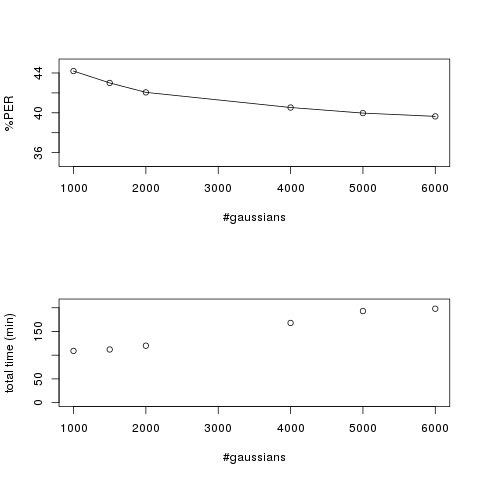
\includegraphics[trim={0 8.5cm 0 0}, clip, width=0.8\linewidth]{chapter03/mono-gaussians.png}
\caption{\textit{Changes in word error rate (\%WER) and phone error rate (\%PER) following variation of the number of total Gaussians allocated to the acoustic model. Scores correspond to decoding performed on the validation set. {\color{red}[TODO]: Add WER + Korean data (WER: 1K:81\%, 3K:77\%, 6K:75\%). Add triphone performance for comparison?}}}
\label{fig:hmm_gaussians}
\end{figure}

\subsection{Language models}
As shown in Figure \ref{fig:hmm_architecture}, the acoustic model is combined with two other components in order to decode speech: the Lexicon and the Language Model (LM).

The lexicon is, put simply, a pronunciation dictionary. It links the acoustic model (i.e., phoneme-level HMMs) with the language model, which is at the word level. For each word, we indicate in the dictionary the sequence of phonemes that constitute it. It is also possible to account for multiple pronunciations of a word due to dialectal differences (e.g., ``tomato'' pronounced as {\color{red}\textipa{/tomeito/} or \textipa{/tomato/}}), phonological phenomena (e.g., homoorganic assimilation: ``handbag'' {\color{red}\textipa{/hanbag/} $\rightarrow$ \textipa{/hambag/}}), or supresegmental information (e.g., stress contrasts: ``record'' \textipa{/'rekord/} (noun) vs. \textipa{/re'kord/} (verb)).

At the word level, the language model stores $P(W)$, the probability of occurrence of word sequences. For this we use \textit{n}-grams: we approximate the probability of a sequence
\begin{equation}
P(W) = P(w_{1})P(w_2|w_1)P(w_3 | w_1, w_2)...P(w_L | w_1, w_2, ..., w_L)
\end{equation}
by the product of the probability of the component words, each conditioned on the \textit{n-1} words preceding it. For instance, if $n = 2$, we obtain a bigram model, where the LM stores the probability of a word depending on a single prceding word. The probability of the word sequence $W$ can then be approximated as:    
\begin{equation}
P(W) \approx P(w_{1})P(w_2|w_1)P(w_3 | w_2)...P(w_L | w_{L-1})
\end{equation}

In our case, these probabilities are obtained from word counts in the training corpus as follows:
\begin{equation}
P(w_i | w_j) \approx \frac{c(w_i, w_j)}{c(w_i)}
\end{equation}
where $c(w_i, w_j)$ is the number of observations of $w_i$ followed by $w_j$, and $c(w_i)$ is the total number of occurrences of $w_i$.
Since not all word combinations are bound to appear in the training corpus, smoothing is performed; null probabilities are given a small probability of appearing. 

Additionally to the bigram word LM, we computed a unigram phone LM in order to evaluate our models' ability to do phonetic decoding. In this case, the lexicon is identical to the phoneme inventory and the LM consists of phoneme counts.  

\subsection{Decoding}
Using dynamic programming, the ASR system builds a graph of the possible word sequences that can serve as transcription of the audio, based on the acoustic model, the lexicon, and the language model. In order to keep the problem computationally tractable, only the most likely transcription hypotheses are kept; this is known as pruning.

\begin{itemize}
\item Lattice generation
\item Acoustic and LM scores 
\item nbest
\item CTM
\item ...
\end{itemize}

\subsection{Scoring: Assessing native performance}

We tested the decoding performance on the validation set of AMs with total number of Gaussians going from 1000 to 6000. We find that the models with the highest amount of Gaussians (i.e., 6000) give the best performance. We did not pursue increasing the number of Gaussians even further, as performance gain was reaching an asymptote at this point and adding more Gaussians would have increased the computational demands for each experiment. Additionally, we expect that adding ``too many'' Gaussians would have lead to overfitting of the models to the training set. Here we provide the evaluation of the Japanese and Korean ASR systems on the test sets ($15\%$ of the corpora), at the lexical level (i.e., using a bigram word LM) and at the phonetic level (i.e., using a unigram phone LM).  

\subsubsection{Lexical decoding}
{\color{red}[TODO] (models currently running)}

\subsubsection{Phonetic decoding}
{\color{red}[TODO] (models currently running)}

%%%%%%%%%%%%
% Parlato2 %
%%%%%%%%%%%%
\newpage
\section{{\color{red}Parlato-hmm}} \label{3-parlato-hmm}
\subsection{Introduction}
\subsection{Methods}
\subsubsection{Stimuli}
We used the same stimuli as in sections \ref{2-parlato} and \ref{2-parlato-dur}. As a reminder, a native French speaker recorded 54 items with the structure $V_{1}C_{1}C_{2}V_{2}$, with $V_{1}$ and $V_{2}$ vowels from the set \{/a/, /i/, /u/\}, and $C_{1}C_{2}$ a cluster from the set \{/bg/, /bn/, /db/, /dg/, /gb/, /gn/\} (e.g. /abgi/).

\subsubsection{Language models}
In order for the decoding task to be analogous to the experiment described in sections \ref{2-parlato_per} and \ref{2-parlato-dur}, trial-specific language models were constructed, as shown in Figure \ref{fig:parlato_G}. Thus, when decoding a $V_{1}C_{1}C_{2}V_{2}$ stimulus, the perception model was only given the possibility to transcribe it as $V_{1}C_{1}(V_{3})(SIL)C_{2}V_{2}$, where phones between parentheses are optional and $V_{3}$ was from the set of vowels \textipa{/a, e, i, o, u/}. In this section our language model was only used to constrain the list of possible outputs from decoding; one output was not more probable than another based on the language models alone. Therefore, here we used a null language model, meaning that the quality of the epenthesized vowels was only determined by the acoustic match.

\begin{figure}[htb]
\centering
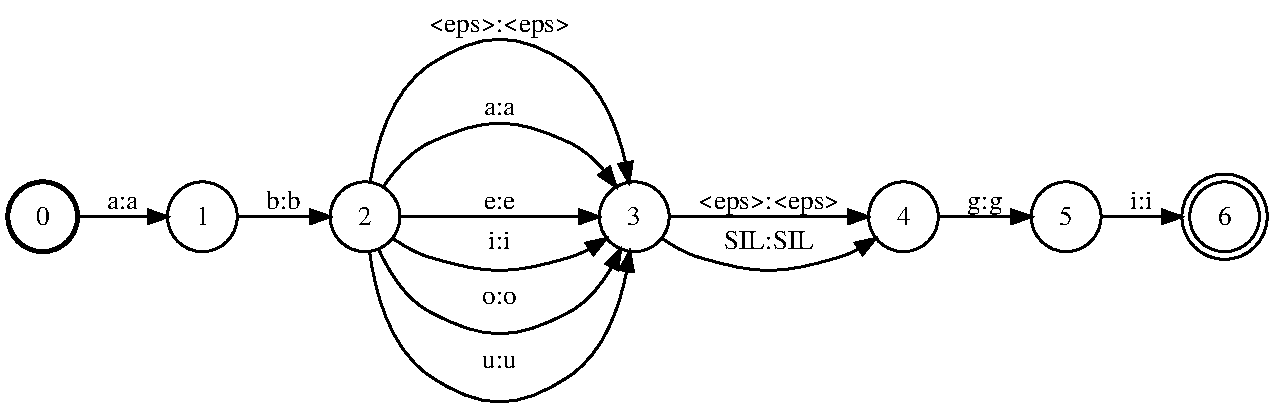
\includegraphics[width=0.8\linewidth]{chapter03/parlato_hmm_Gfst.pdf}
\caption{Constrained language model used for decoding the stimulus \textipa{/agni/}. Nodes in the graph represent states, edges represent transitions between states (here: phonemes). The lack of weights on edges issued from a same node (e.g., between states 2 and 3) indicates that path selection is entirely decided by acoustic scores when decoding experimental items, with an acoustic scale of $0.1$. An optional silence can be inserted by the model between states 3 and 4.}
\label{fig:parlato_G}
\end{figure}

\subsubsection{Identification task simulation}
After decoding the stimuli, we obtained for each possible transcription of each item the corresponding acoustic and language model scores. An example of how the ASR system decodes the experimental stimuli can be seen in Figure \ref{fig:parl_hmm_align}. From the acoustic and language model scores\footnote{with an acoustic scale of $0.1$} we derived the item posteriorgrams, which indicate how probable a given transcription was given the audio input. We used these probabilities as proxies of the probability that a listener might exploit when performing reverse inference during speech perception, and therefore, the probabilities used when responding in an identification task. 

As such, for each item, we obtained a six-dimensional vector $ident_{model} = [p_{none}, p_{a}, p_{e}, p_{i}, p_{o}, p_{u}]$, containing a discrete probability distribution, with a probability mass function linking the identification task options `none', `a', `e', `i', `o', `u', to their respective probabilities (i.e., posteriorgrams).
We can define the human equivalent $ident_{human} = [p_{none}, p_{a}, p_{e}, p_{i}, p_{o}, p_{u}]$, which contains the percentage of responses for each item, after aggregating all participant responses. 

\begin{figure}[htb!]
  \centering
  \begin{overpic}[trim={0 2.5cm 0 1.5cm},clip, width=0.8\linewidth]{chapter03/parlato-hmm_praat_agni.pdf}\end{overpic}
  \caption{\textit{Example of how the ASR system decodes the item \textipa{/agni/}, using the null language model in Figure \ref{fig:parlato_G}. From top to bottom: original waveform, item name, aligned transcriptions given by the model (from the most probable to the least probable), and spectrogram with formant contours. SIL = silence.}}
  \label{fig:parl_hmm_align}
\end{figure}

\subsubsection{Data analysis}
Statistical analyses were performed with the R statistical software \cite{R-base}, using Markov chain Monte Carlo generalised linear mixed-models \cite{R-MCMCglmm, R-coda}. These Bayesian models sample coefficients from the posterior probability distribution conditioned on the data and given priors. We used priors that are standard for linear models. Model convergence was assessed by visual inspection of trace plots and the Gelman–Rubin convergence diagnostic \cite{gelman1992}, using eight chains with different initialisations. Effects were considered statistically significant if the 95\% highest posterior density (HPD) interval estimated for the coefficient of interest did not include zero. We report both the posterior mode and the 95\% HPD interval.  

In order to assess the influence of $V_{1}$ and $V_{2}$ (henceforth: flanking vowels) on epenthetic vowel quality (/i/ or /u/), we chose as fixed effect for our statistical models \textsc{Number of Same Flanking Vowels} (\textsc{NSFV}; considered as a continuous variable with values 0, 1, or 2 instead of a factor with 3 levels, in order to reduce the number of model parameters and promote convergence). Due to the almost null variance and the consequent poor trace plot for the random intercept \textsc{Cluster}, we did not include it in the statistical models. Our response variable was the continuous variable \textsc{Posteriorgram}.\footnote{Responses by human participants and exemplar models were given by trial; therefore in previous analyses the response variable was binomial.}

\subsection{Results}
\subsubsection{Overall similarity}
\begin{figure}[H]
  \centering
  \begin{overpic}[trim={0 0 0 0.75cm}, clip, page=1, width=0.5\linewidth]{chapter03/parl_hmm_figs}\end{overpic}
  \caption{\textit{Distribution of posteriorgrams obtained when decoding with a null language model. The box and whiskers plots display the distribution of posteriorgrams across experimental items.}}
  \label{fig:parl_hmm_overall}
\end{figure}
Figure \ref{fig:parl_hmm_overall} shows the distribution of posteriorgrams for each response, with one datapoint per stimulus. The most probable transcriptions for the stimuli were ``none'' (26.7\%), ``u'' (24.3\%) and ``i'' (22.5\%).  While these were also the most frequent responses given by human participants (``none'': 13.1\%; ``u'': 63.1\%; ``i'': 15.3\%), the preponderance of \textipa{/u/}-epenthesis is missing in the model.

% > agr.ep (model average pgram)
%   resp          x
% 1 none 0.26667043
% 2    a 0.04802057
% 3    e 0.12948173
% 4    i 0.22494707
% 5    o 0.08715853
% 6    u 0.24372167

% > colMeans(d.comp.per[-1]) (human average resp)
%     p.none        p.a        p.e        p.i        p.o        p.u 
% 0.13071895 0.01416122 0.02505447 0.15250545 0.04684096 0.63071895 

In order to have a general idea of the model's ability to reproduce human behaviour, we computed the distance between human and model response patterns by computing the normalized Euclidean distance between $ident_{model}$ and $ident_{human}$, within each experimental item. The mean (and median) distance was $0.44$. This is higher than what was obtained by the best exemplar model in section \ref{2-parlato-dur} (mean distance: $0.33$; median distance: $0.21$); however remember that exemplar models were only able to output ``i'', ``o'', and ``u'' as responses. When computing the distance by taking into account the missing responses ``none'', ``a'', and ``e'', responses from the best JP exemplar model have a mean distance of $0.39$ (median: $0.30$) with respect to human responses.

While it might be tempting to conclude that the exemplar model was superior compared to the HMM model, it is important to note that the task modelled by the HMM-based model is closer to the task participants were subjected to (6-alternative forced choice identification task) than the exemplar models (3-AFC identification task). Technically, a ``dummy'' model in the 3-AFC situation, where all options are equally probable, would output ``u'' for $33\%$ of the trials. This is a higher percentage of \textipa{/u/}-epenthesis than the $24.3\%$ from our current model. Since ``u'' is by far the most frequent response given by human participants (and ``a'' and ``e'' are very infrequent), even a dummy 3-AFC \textipa{\{``i'', ``o'', ``u''\}} model might outclass our 6-AFC \textipa{\{``none'', ``a'', ``e'', ``i'', ``o'', ``u''\}} ASR system.

As such, we believe that it is unfair to compare Euclidean distances between models based on different tasks. We can, however, see if the ASR-based model reproduces the qualitative effects that the best exemplar model was able to mimic.

\subsubsection{Effect of coarticulation}

\paragraph{/i/-epenthesis}

The left panel of Figure \ref{fig:parl_hmm_iu} shows the posteriorgrams for \textipa{/i/}-epenthesis given by our ASR-based model with a ``null'' language model.
The main effect of \textsc{NSFV} was significant (mode: $0.10$, HPD: $[0.01, 0.18]$). An increased number of \textipa{/i/} flanking vowels resulted in higher posteriorgrams for stimuli transcriptions with \textipa{/i/} epenthesis.

\begin{figure}[H]
  \centering
  \begin{overpic}[page=2, width=0.4\linewidth]{chapter03/parl_hmm_figs}\end{overpic}
  \hspace{1cm}
  \begin{overpic}[page=3, width=0.4\linewidth]{chapter03/parl_hmm_figs}\end{overpic}
  \caption{\textit{Posteriorgrams for \textipa{/i/}-epenthesis (left) and \textipa{/u/}-epenthesis (right) obtained when decoding with a ``null'' language model. The box and whiskers plots display the distribution of posteriorgrams across experimental items, represented by individual dots.}}
  \label{fig:parl_hmm_iu}
\end{figure}

\paragraph{/u/-epenthesis}
The right panel of Figure \ref{fig:parl_hmm_iu} shows the posteriorgrams for \textipa{/u/}-epenthesis given by our ASR-based model with a ``null'' language model.
The main effect of \textsc{NSFV} was not significant (mode: $0.04$, HPD: $[-0.02, 0.10]$). Therefore, an increased number of \textipa{/u/} flanking vowels did not result in significantly higher posteriorgrams for stimuli transcriptions with \textipa{/u/} epenthesis.

\subsection{Discussion}
%%% Summary

%%% Duration in ASR? [check topology]

%%%%%%%%%%%%%%%%%%%%%%%%%%
% m-/ahpa/ + parlato_lms %
%%%%%%%%%%%%%%%%%%%%%%%%%%
\newpage
\section{{\color{red}Investigating surface phonotactics}} \label{3-surfphono}

\small{\textit{{\color{red}ADD ACKNOWLEDGEMENTS THOMAS + EMMANUEL.\\}}}

\subsection{Introduction}
\subsection{Experiment 1: {\color{red}Parlato-lms}}
\subsubsection{Methods}
\paragraph{Stimuli}
We used the same stimuli as in sections \ref{2-parlato}, \ref{2-parlato-dur}, and \ref{3-parlato-hmm}. As a reminder, a native French speaker recorded 54 items with the structure $V_{1}C_{1}C_{2}V_{2}$, with $V_{1}$ and $V_{2}$ vowels from the set \{/a/, /i/, /u/\}, and $C_{1}C_{2}$ a cluster from the set \{/bg/, /bn/, /db/, /dg/, /gb/, /gn/\} (e.g. /abgi/).

\paragraph{Language models}
In this section, we investigate the type of phonotactic information that might be used by Japanese listeners when perceiving foreign speech that does not conform to native phonotactics. We test 5 types of language models (LM) when decoding our $V_{1}C_{1}C_{2}V_{2}$ items; these differ only in the weights given to edges between nodes 2 and 3 in the graph shown in Figure \ref{fig:parlato_G}. 
\begin{enumerate}
    \item A null language model, which implies that listeners base their decoding of consonant clusters on phonetics alone, without using information on phonotactics (as in section \ref{3-parlato-hmm}).
    \item A phone-unigram language model, which implies that listeners do not take neighbouring phonemes into consideration when decoding the consonant clusters; only the frequency of the vowel $V_{ep}$ to be epenthesized (compared to that of $C_{2}$) is taken into account when choosing epenthetic vowel quality.
    \item An online phone-bigram language model, which implies that listeners decode the clusters as they hear them (decoding is done from the start of the item). Here the choice of epenthetic vowel is modulated by $C_{1}V_{ep}$ and $C_{1}C_{2}$ diphone frequencies. 
    \item A retro phone-bigram language model, which implies that listeners decode the clusters based on the most recent information (decoding is done from the end of the item). Here the choice of epenthetic vowel is modulated by $V_{ep}C_{2}$ and $C_{1}C_{2}$ diphone frequencies.
    \item A batch phone-bigram language model, which implies that listeners decode the item considering the entire structure, with bigrams. Here the choice of epenthetic vowel is modulated by $C_{1}V_{ep}$ and $V_{ep}C_{2}$ (and $C_{1}C_{2}$) diphone frequencies.  
\end{enumerate}

The weights, which can be found in Table \ref{}, were obtained by taking frequency counts from the portion of the CSJ used for training the acoustic model: 
{\color{red}ADD TABLE WITH FREQUENCIES}


\paragraph{Identification task simulation}
We used the same procedure as in section \ref{3-parlato-hmm}. Therefore, for each LM, we obtain for each item a six-dimensional vector $ident_{LM} = [p_{none}, p_{a}, p_{e}, p_{i}, p_{o}, p_{u}]$ containing posteriorgrams for each of the six possible responses. In a similar way, the human equivalent $ident_{human} = [p_{none}, p_{a}, p_{e}, p_{i}, p_{o}, p_{u}]$ contains the percentage of responses for each item, after aggregating all participant responses. 

\paragraph{Data analysis}
In order to compare how well LMs compared at mimicking human behaviour, we computed the Euclidean distance between $ident_{LM}$ and $ident_{human}$ for each item, for each LM. Do models that integrate information about phoneme probabilities (i.e., \textsc{unigram} LM) or diphone probabilities (i.e., \textsc{bigram} LMs) show smaller \textsc{Eucl. distances} to human data than the \textsc{null} LM?

The response variable of our statistical models was the \textsc{Eucl. distance} between $ident_{LM}$ and $ident_{human}$, as described above.  
We chose as fixed effect the \textsc{Language Model} (\textsc{LM}) used during decoding, considered as a categorical variable with \textsc{null} as the reference level. The variable was contrast coded with simple coding, meaning that non-reference levels were compared to the reference level, with the intercept corresponding to the grand mean (all levels).
\textsc{$C_{1}$} was added as a random intercept.

Statistical analyses were performed with the R statistical software \cite{R-base}, using Markov chain Monte Carlo generalised linear mixed-models \cite{R-MCMCglmm, R-coda}. These Bayesian models sample coefficients from the posterior probability distribution conditioned on the data and given priors. We used priors that are standard for linear models. Model convergence was assessed by visual inspection of trace plots and the Gelman–Rubin convergence diagnostic \cite{gelman1992}, using eight chains with different initialisations. Effects were considered statistically significant if the 95\% highest posterior density (HPD) interval estimated for the coefficient of interest did not include zero. We report both the posterior mode and the 95\% HPD interval.  

%\begin{itemize}
%\item \textsc{\%none}: Proportion of ``none'' responses (no epenthesis) over all trials.
%\item \textsc{\%$V_{1}\underline{\vee}V_{2}$}: Proportion of trials where the epenthesized vowel shares the quality of either $V_{1}$ or $V_{2}$, with $V_{1} \neq V_{2}$ (out of all trials with epenthesis).
%\item \textsc{\%$V_{1}\land V_{2}$}: Proportion of trials where the epenthesized vowel shares the quality of both $V_{1}$ and $V_{2}$, with $V_{1} = V_{2}$ (out of all trials with epenthesis).
%\item \textsc{\%default}: Proportion of default \textipa{/u/}-epenthesis over all trials
%\item \textsc{\%coronal}: Proportion of \textipa{/o/}-epenthesis following coronal consonants over all trials with clusters containing coronal consonants 
%\end{itemize} 

\subsubsection{Results and Discussion}
\begin{figure}[htb!]
    \centering
    \includegraphics[page=2, width=0.8\linewidth]{chapter03/parlato-lms_figs.pdf}
    \caption{\textit{Distribution of the proportion of responses given by human participants (topmost panel) and posteriorgrams obtained when decoding with different language models. The box and whiskers plots display the distribution of posteriorgrams across experimental items, with boxplots separated according to the $C_{1}$ in the cluster.}}
    \label{fig:parlato-lms}
  \end{figure}
  
\paragraph{Effect of acoustic scale}

\paragraph{Response patterns}
{\color{red}Graph showing response patterns}


\paragraph{Overall similarity}
We found that, relative to the \textsc{null} LM, the \textsc{bigram online} (mode: $0.08$, HPD: $[0.02, 0.15]$) and the \textsc{bigram batch} (mode: $0.08$, HPD: $[0.02, 0.15]$) language models resulted in significantly higher Euclidean distances between the model responses and human responses. On the other hand, we did not find evidence of a difference between the \textsc{null} LM and the \textsc{unigram} (mode: $0.03$, HPD: $[-0.04, 0.10]$) or \textsc{bigram retro} (mode: $0.0$, HPD: $[-0.06, 0.07]$) language models.

\paragraph{Zooming in on epenthetic vowel quality}
We arbitrarily chose a smoothing factor ($10^{-8}$)  in order to allow the language models to assign a non-zero probability to diphones never seen in the language corpus. The magnitude of this smoothing factor is expected to have an effect on the posteriorgrams assigned to ``none'' responses when decoding the experimental items. Since ``none'' responses constitute $13\%$ of human responses, and since the choice of the smoothing factor only affects the bigram language models, it may be beneficial to do a post-hoc analysis focusing on the models' ability to mimic epenthetic vowel quality after isolating it from the percentage of epenthesis. As such, we perform the same analysis as above, but after removing $p_{none}$ from $ident_{LM}$ and $ident_{human}$.

The results are qualitatively identical: relative to the \textsc{null} LM, only the \textsc{bigram online} (mode: $0.11$, HPD: $[0.05, 0.19]$) and the \textsc{bigram batch (2PB)} (mode: $0.11$, HPD: $[0.05, 0.19]$) language models resulted in significantly higher Euclidean distances. There was no evidence of a significant difference for the \textsc{unigram (1P)} (mode: $0.06$, HPD: $[-0.02, 0.12]$) or \textsc{bigram retro (2PR)} (mode: $0.03$, HPD: $[-0.04, 0.10]$) language models 

Interestingly, the models that performed less similarly to human behaviour are those for which \textipa{/u/}- and \textipa{/i/}-epenthesis was blocked after coronal consonants, since \textipa{/du/} and \textipa{/di/} are phonotactically illegal in Japanese and therefore do not appear in our corpus. Yet, as seen in Figure \ref{fig:parlato_per_all}, JP participants mostly reported experiencing \textipa{/u/}- and \textipa{/i/}-epenthesis on trials where $C_{1}$ was a coronal consonant. Similar to how ``none'' responses are blocked for all bigram models, acoustics are unable to counter the low diphone probability of \textipa{/du/} and \textipa{/di/}.

\subsection{Experiment 2: {\color{red}m-/ahpa/}}
\subsubsection{Methods}
\paragraph{Stimuli}
We used the same stimuli as in section \ref{2-ahpa}. As a reminder, we recorded 3 speakers producing disyllabic $V_{1}C_{1}C_{2}V_{1}$ and trisyllabic $V_{1}C_{1}V_{2}C_{2}V_{1}$, with $V_{1}$ a flanking vowel in the set \textipa{/a, e, i, o, u/}, $C_{1}$ \textipa{/h/} or /k/, and $C_{2}$ a fixed consonant, /p/ (e.g, \textipa{/ahpa/}, \textipa{/ahapa/}). By cross-splicing the disyllabic natural control items (e.g., \textipa{/ahpa/}), we obtained disyllabic spliced control items (e.g., \texorpdfstring{\textipa{/ah\textsubscript{a}pa/}}{}), disyllabic spliced test stimuli (e.g., \texorpdfstring{\textipa{/ah\textsubscript{u}pa/}}{}), and trisyllabic spliced fillers (e.g., {\textipa{/ahapa/}), where subscripts indicate the identity of the vowels flanking the clusters in the original recording. Therefore, within each speaker, all stimuli of the same structure (in our example, \textipa{/ah($V$)pa/} items) are acoustically identical on their flanking vowels.
  
\paragraph{Language models}
We used the same language models as in Experiment 1, adapted to the $V_{1}C_{1}C_{2}V_{1}$ items used in this experiment. A graphical representation can be found in Figure \ref{fig:m-ahpa_G}.
  
\begin{figure}[htb]
    \centering
    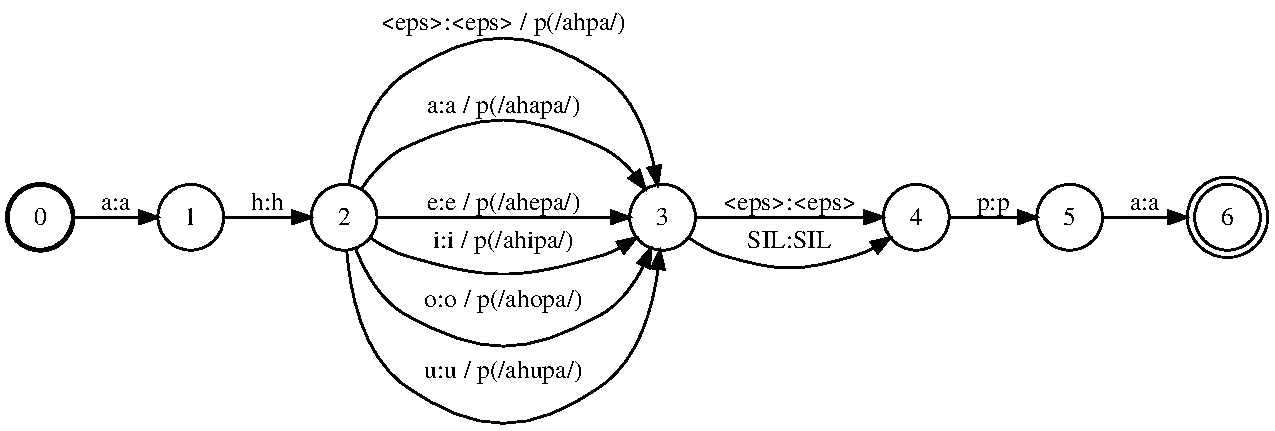
\includegraphics[width=0.8\linewidth]{chapter03/m-ahpa_Gfst.pdf}
    \caption{\textit{Constrained language model used to test the models (here: LM for \textipa{/ahpa/} trials). Nodes in the graph represent states, weighted edges represent transitions between states (here: phonemes). When relevant, weighted edges are labeled with the probability to choose that edge when decoding, which affects the final language model score of each possible path. These scores are then combined with acoustic scores when decoding experimental items.}}
    \label{fig:m-ahpa_G}
\end{figure}
  
\paragraph{Identification task simulation}
We used the same procedure as in section \ref{3-parlato-hmm}.

\paragraph{{\color{red}Data analysis}}
% Refer to previous experiment
% Model selection
% Parameter tuning

%In order to select the language model which best predicted our behavioural data, we inferred the \textit{a posteriori} distributions of the weights given to acoustic model and language model in {\color{red}equation \ref{}}, using ABC. The following aggregated data were used as summary statistics:

%\begin{itemize}
%\item \textsc{\%none}: Proportion of ``none'' responses (no epenthesis)
%\item \textsc{\%coart}: Proportion of trials where the epenthesized vowel shares the quality of the coarticulation within the consonant (including \textipa{/u/} coarticulation).
%\item \textsc{\%default}: Proportion of default \textipa{/u/}-epenthesis over all trials
%\end{itemize}

%Since we saw in section \ref{2-ahpa} that patterns of epenthesis differed depending on whether the consonant cluster was \textipa{/hp/} or \textipa{/kp/}, we computed these summary statistics twice, one set per consonant cluster. As such, the final number of statistics was six. 

\subsubsection{Results and Discussion}
\subsection{Discussion}

%%%%%%%%%%%%
% k-epenth %
%%%%%%%%%%%%
\newpage
\section{{\color{red}Do we need to go deeper? Are surface phonotactics enough?}} \label{3-k-epenth}
\subsection{Introduction}
\subsection{Methods}
\subsubsection{Stimuli}

The stimuli, which have been previously used in \cite{durvasula2015}, were kindly provided by the authors from said paper. They consist of 12 items of the form \textipa{/e}C(V)\textipa{ma/}, with \textsc{C} either an alveolar consonant from the set \{\textipa{/t\super h, s/}\} or a palatal consonant from the set \{\textipa{c\super h, S/}\}, and \textsc{V} a vowel from the set \{\textipa{/1}\footnote{Following the original article, we use \textipa{[1]} to denote the close back unrounded vowel. However, the notation \textipa{[W]} has also previously been used (e.g., in \cite{kabak2007})}\textipa{, i/}\}.
Each item was recorded twice by a male trained phonetician. The speaker is a native speaker of Indian English and Telugu, also a near-native speaker of standard Hindi. The clusters present in the items are phonotactically legal in these two latter languages. All items were produced with stress on the first syllable.
The organisation of the stimuli, based on place of articulation of \textsc{C}, is shown on Table \ref{tab:k-ep_stim}.

\begin{table}[htb!]
\centering
\caption{\textit{Experimental items. Reproduced from \cite{durvasula2015} (Table I).}}
\label{tab:k-ep_stim}
\begin{tabular}{c|c|c|c|c}
  \cline{2-4}
         & \multicolumn{3}{c|}{vowels} &  \\ \cline{2-4}
         & \textipa{[1]}         & \textipa{[i]}    & none    &  \\ \cline{1-4}
  \multicolumn{1}{|l|}{alveolar} & \textipa{et\super h1ma}     &  \textipa{et\super hima}    &  \textipa{et\super hma}       &  \\ \cline{2-4}
  \multicolumn{1}{|l|}{}       &  \textipa{es1ma}         &  \textipa{esima}    &  \textipa{esma}       &  \\ \cline{1-4}
  \multicolumn{1}{|l|}{palatal}  &  \textipa{ec\super h1ma}          &  \textipa{ec\super hima}     &  \textipa{ec\super hma}        &  \\ \cline{2-4}
  \multicolumn{1}{|l|}{}                       &  \textipa{eS1ma}         &  \textipa{eSima}    &  \textipa{eSma}       & \\ \cline{1-4} 
\end{tabular}
\end{table}

\paragraph{Language models}

\paragraph{Identification task simulation}


\subsubsection{Data analysis}
\subsection{Results}
\subsection{Discussion}
%%%%%%%%%%%%%%%%%%%%%%%%%%%
% Chapter mini-discussion %
%%%%%%%%%%%%%%%%%%%%%%%%%%%
\section{Conclusions}
%%% Summary

%%% Short discussion

%%% Limitations

%%% Conclusions